\section{Results}
\label{sec:results}

\begin{figure}
  %% \labresults{Single-point distributions}%
  %%            {figures/point-distributions-cropped.pdf}
  %% \begin{center}
  %%   $\begin{array}{r|c@{~}c|}
  %%   \multicolumn{1}{c}{}
  %%   & P(\kappa=1)
  %%   & \multicolumn{1}{c}{P(\kappa=2)}
  %%   \\ \cline{2-3} 1 & 0.005 & 0.0005
  %%   \\ 2 & 0.01  & 0.001
  %%   \\ 3 & 0.05  & 0.005
  %%   \\ 4 & 0.1   & 0.01
  %%   \\ \cline{2-3}
  %% \end{array}$
  %%   \hspace{\fill}
  %%   $\begin{array}{r|c@{~}c|}
  %%   \multicolumn{1}{c}{}
  %%   & P(\kappa=1)
  %%   & \multicolumn{1}{c}{P(\kappa=2)}
  %%   \\ \cline{2-3} 5 & 0.25  & 0.125
  %%   \\ 6 & 0.33333 & 0.22222
  %%   \\ 7 & 0.375 & 0.28125
  %%   \\ 8 & 0.46875 & 0.439453125
  %%   \\ \cline{2-3}
  %% \end{array}$
  %% \end{center}
  \[
\begin{array}{cc|cc|cc}
\\  & %\multicolumn{1}{c}{} 
    & \multicolumn{2}{c}{s2a=3} & \multicolumn{2}{c}{s2a=2}
\\  \multicolumn{1}{c}{P(\kappa=1)} & \multicolumn{1}{c|}{P(\kappa=2)} & \multicolumn{1}{c}{P} & \multicolumn{1}{c}{R} & \multicolumn{1}{c}{P} & \multicolumn{1}{c}{R}
\\ \hline
   0.005   & 0.0005   & 99.97 & 96.73 & 99.28 & 98.32
\\ 0.01    & 0.001    & 99.93 & 96.39 & 98.81 & 98.04
\\ 0.05    & 0.005    & 96.36 & 92.94 & 94.37 & 97.33
\\ 0.1     & 0.01     & 86.71 & 89.47 & 89.92 & 96.23
\\ 0.25    & 0.125    & 84.16 & 56.93 & 74.53 & 70.57
\\ 0.33333 & 0.22222  & 75.87 & 39.52 & 66.06 & 53.78
\\ 0.375   & 0.28125  & 71.56 & 31.28 & 61.84 & 45.34
\\ 0.46975 & 0.43945  & 58.57 & 15.54 & 53.56 & 27.76
\\ \hline
\end{array}
\]


%%% Local Variables: 
%%% mode: latex
%%% TeX-master: "../main"
%%% End: 

  \caption{Precision (P) and recall (R) percentages from the \textbf{varying
      probabilities} experiment.  The second result set varies
    the initial sensor-to-attack ratio (s2a) from 3 to 2.
    %%
    %% The lower key relates the labels on the x axis to assignments
    %% of probabilities to kappas. $P(\kappa = 0) = 0.5$ for all.
  }
  \label{fig:vary-kappa-results}
\end{figure}

%% IN JOURNAL VERSION --- smoothed vs. unsmoothed results; see
%% also commented-out lines in figures/vary-kappas-beta-unified.gip
\begin{figure}
    \labresults{(i) Beta distributions}{figures/vary-kappas-beta-unified-cropped.pdf}
%%  \caption{Precision and recall percentages for the \textbf{non
%%      point-value distribution} experiment. 
%%    %The mean values of the
%%    %distributions translating $\kappa(0)$, $\kappa(1)$ and $\kappa(2)$
%%    %are respectively $0.5$, $0.01$ and $0.001$; the sample sizes
%%    %$\alpha+\beta$ vary as shown.
%%  }
%%  \label{fig:vary-beta-results}
%%\end{figure}
%%\begin{figure}
\\  \labresultsT{(ii) Sensor imprecision}{figures/crowding-sensors-cropped.pdf}
%%  \caption[Precision and recall percentages of the \textbf{crowding
%%      sensors} experiment.]%
%%          {Precision and recall percentages of the
%%  \textbf{crowding sensors} experiment.}
%%  \label{fig:vary-crowding-results}
%%\end{figure}
%%\begin{figure}
\\  \labresultsT{(iii) Base rate}{figures/base-rate-cropped.pdf}
%%  \caption{Precision and recall percentages of the \textbf{base rate}
%%    experiment.}
%%  \label{fig:vary-baserate-results}
\caption{Precision and recall percentages for the \textbf{beta
    distribution}, \textbf{sensor imprecision} and \textbf{base rate}
  experiments. }
  \label{fig:vary-beta-results}
  \label{fig:vary-crowding-results}
  \label{fig:vary-baserate-results}
\end{figure}

\begin{figure*}
  \centering
  \textsf{Three sensors}\hspace{40mm}\textsf{Two sensors}
  \hspace{38mm}\textsf{Single sensor} 
  \\
  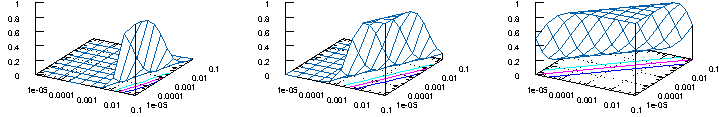
\includegraphics[width=\textwidth]{figures/consolidated-base-rate-cropped.pdf}
  \caption[Base rate problems and sensor fusion.]
%%
    {Graphs of quantitative false positive probabilities (on the
      z-axis) as function of the probability of an individual sensor
      giving a false positive reading (on the x-axis, running from the
      origin to the lower right on each graph) and attack probability
      (on the y-axis).  Specifically, each graph plots
      $z=P(\mathrm{no~attack}|\mathrm{alarm~raised})=\frac{x^s(1-y)}{y+x^s(1-y)}$
      for the given number of sensors $s$. }
    %%{Base rate problems and sensor fusion.  The graphs show the false
    %%  positive probabilities (on the z-axis) as a function of the
    %%  false alarm probability (on the x-axis, running from the origin
    %%  to the lower right on each graph) and attack probability (on the
    %%  y-axis).  The diagonal contour lines project onto the xy-plane
    %%  where the surface intersects z=0.25, z=0.5 and z=0.75.}
  \label{fig:base-rate-plots}
\end{figure*}


\emph{Varying probabilities.}
Figure~\ref{fig:vary-kappa-results} shows \mifd's performance as the
stratified likelihood rankings become less distinct.
We see that MIFD's performance degrades gracefully as the probabilities
corresponding to $\kappa(0), \kappa(1)$ and $\kappa(2)$ approach each other.
Although the
theoretical basis of the qualitative probability levels is
infinitesimal, \mifd\ performs reasonably for $P(\kappa=1)$ and
$P(\kappa=2)$ taken as high as 0.05 and 0.005 respectively.
\mifd\ also degrades gracefully as its input sensors become
less discriminating, simulated by raising the sensor-to-attack ratio
from 2 to 3.  We had expected \mifd\ to be more brittle under
sensor-to-attack ratio 2, but this was only partly true;
precision declines more quickly with ratio 2 than with ratio 3.
Recall declines less quickly, because the corroboration of several
sensors
is more relevant to suppressing spurious additional event diagnoses.


\emph{Non point-value distributions.}
Figure~\ref{fig:vary-beta-results}\,(i) shows \mifd's performance when we
interpret the qualitative likelihood levels as various beta
distributions.
The results confirm those of the previous experiment, and show that MIFD is not sensitive
to variance in the probabilities of events at the same qualitative surprise level.

\emph{Sensor imprecision.}
Figure~\ref{fig:vary-crowding-results}\,(ii) shows how \mifd's accuracy
declines when sensors correspond to more than one event.  
Recall and precision stay well above 90\% for sensors responding to
two or fewer distinct events. Unsurprisingly, precision declines sharply as
sensors respond to three or more events.  This decline is not
particularly serious in practice: actual \ids\ sensors rarely detect
large numbers of events: if they do we introduce new
abstractions.

\emph{Base rate.} \label{sec:base-rate}
Figure \ref{fig:base-rate-plots} shows the challenge of base rates, and how MIFD
addresses it through sensor fusion.  
In the rightmost plot, we see
that the
false positive probability is extremely high with only one sensor, even a very
accurate
one.  However, requiring corroboration from two or three sensors,
as MIFD does, reduces the false alarm rate substantially.
Note that this requires the sensors to fail independently.  If sensors'
false positives are correlated, then corroboration can fail to
lower the false positive rate.  It was
to handle such correlated failures that we introduced benign events
into Scyllarus and MIFD.


Figure~\ref{fig:vary-baserate-results}\,(iii) shows how \mifd's false
positive rate rises with event rarity. The high recall shows that
\mifd\ does find the attacks (the bounce up at the right is because of the
extremely low sample size), but declining precision is from mistakenly
hypothesizing additional attacks.  Precision declined unacceptably
below 90\% for smaller attack probabilities
than shown on this chart.

% LATER: What accounts for the oddball results here?

%%% Local Variables: 
%%% mode: latex
%%% TeX-master: "main"
%%% End: 
